
\subsection{Recherche documentaire}
\subsubsection{AutoBiomes: procedural generation of multi-biome landscapes (2020) \cite{Autobiome}}
    
    
    \paragraph{Approche proposée pour la génération procédurale de terrains}
    Les auteurs présentent un système de génération procédurale de terrain combinant trois types d’approches : synthétique, physique et exemple-based (basée sur des exemples). L’objectif est de créer des paysages étendus, composés de différents biomes et peuplés de nombreux éléments.
    
    Le système repose sur un pipeline, structuré en quatre étapes principales. Chaque étape peut être visualisée directement, ce qui améliore la facilité d’utilisation.Chaque étape est placée sur une grille comme présenté dans le figure ci dessous. Ce design offre un bon compromis entre les exigences souvent opposées : performance, réalisme, flexibilité. Voici les différentes étapes de ce pipeline:

    \begin{figure}[!h]
    \centering
    \begin{subfigure}{0.4\linewidth}
        \centering
        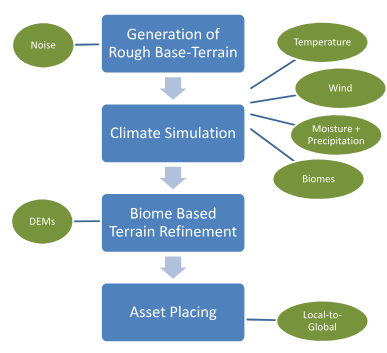
\includegraphics[width=\linewidth]{images/pipeline_autobiomes.png}
        \caption{Pipeline présenté dans le papier}
        \label{fig:image_avant_expansion}image
    \end{subfigure}
    \hfill
    \begin{subfigure}{0.4\linewidth}
        \centering
        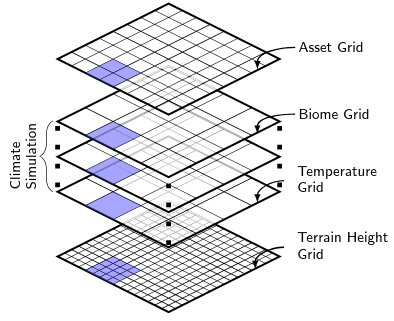
\includegraphics[width=\linewidth]{images/grille_autobiomes.png}
        \caption{Structure de grilles utilisé pour la génération}
        \label{fig:histo_avant_expansion}
    \end{subfigure}
    \caption{Images tirés du papier}
\end{figure}

    \paragraph{Terrain de Base}
    Généré à l’aide de fonctions de bruit, notamment du simplex noise multi-octaves. Cela permet une création rapide et flexible d’un terrain général, sans se soucier des détails réalistes dès cette étape. L'utilisateur peut ajuster les paramètres, comme le nombre d'octaves ou le seuil de niveau de la mer.


    \paragraph{Simulation climatique}
    Cette étape a pour but de calculer la distribution des biomes la plus réaliste possible. Pour cela aucun bruit n'est utilisé mais une approche basée sur la physique a été choisie elle reste simple pour qu'elle soit relativement rapide contrairement a d'autres méthodes basées sur la simulation physique. Elle se compose de 4 étapes:
    \begin{itemize}
        \item \textbf{Température}: Calculée par interpolation bilinéaire ou sinusoïdale, en prenant en compte l’altitude (plus c’est haut, plus c’est froid). Cela permet d'avoir un gradient entre régions chaudes et froides.
        
        \item \textbf{Vent}: Le vent est simulé en définissant des forces aux quatre coins de la carte. Une approche itérative propage les directions de vent dans un champ vectoriel, en combinant les directions des cellules voisines et en ajoutant de petites perturbations aléatoires pour simuler les micro-variations. La proximité d’un coin renforce la persistance de son influence, produisant ainsi un lissage réaliste ou des annulations aux frontières entre courants principaux.
        
        \item \textbf{Précipitations}: La répartition des précipitations est calculée de manière itérative, en utilisant les données de vent et de température. Les cellules d’eau servent de sources d’humidité, avec une évaporation dépendant de la température. L’humidité est ensuite transportée par le vent vers les cellules voisines, avec une dispersion partielle vers les cellules adjacentes. Cette méthode permet de de simuler des phénomènes plus avancés comme les ombres pluviométriques ou l'effet de foehn.

        \item \textbf{Placement des biomes}: Calcul de la grille de Biomes en fonction des propriétés calculées, en particulier la température et les précipitations. À chaque paire de valeurs température-précipitation est ainsi associé un identifiant de biome spécifique, selon une table.
    \end{itemize}
    
    \paragraph{Enrichissement du terrain}: Pour enrichir le terrain de base, les auteurs utilisent une approche par exemple en intégrant des DEMs (modèles numériques d'élévation) spécifiques à chaque biome, tirés de sources disponibles publiquement. Les DEMs sont une représentation numérique de la hauteur du terrain sur une surface donnée, généralement sous forme d'une grille régulière où chaque cellule contient une valeur d'altitude. Cette méthode offre un réalisme élevé avec peu d’efforts.
    Pour obtenir des transitions naturelles entre biomes, les frontières sont déformées avec du bruit fractal (simplex noise), générant une grille de biomes à plus haute résolution. Ensuite, une convolution avec un noyau réglable permet de mélanger les DEMs voisins selon la proportion de chaque biome dans la zone. Le résultat est une somme pondérée des DEMs, fusionnée au terrain de base pour produire une carte de hauteur finale réaliste et cohérente.

    \paragraph{Placement d'objets}: Dans la dernière étape, les biomes sont peuplés par des objets 3D (assets) placés selon un modèle itératif. Ce modèle permet des distributions naturelles et adaptables aux transitions entre biomes. Les objets sont sélectionnés depuis une base d’assets (arbre, rocher, etc.), chacun possédant des propriétés spécifiques (ex. : tolérance à l’ombre, distance minimale, etc.).
    Le placement se fait via un échantillonnage de type Poisson-disk, adapté pour gérer des distributions complexes avec contraintes. Les objets sont traités par catégories (organique/inorganique, petite/grande taille) pour une répartition plus réaliste. On obtient une répartition uniforme et performante d'objets dur le terrain généré.
    

    \paragraph{Résultats obtenus}
    Voici les résultats présentés par les auteurs:
    \begin{figure}[!h]
        \centering
        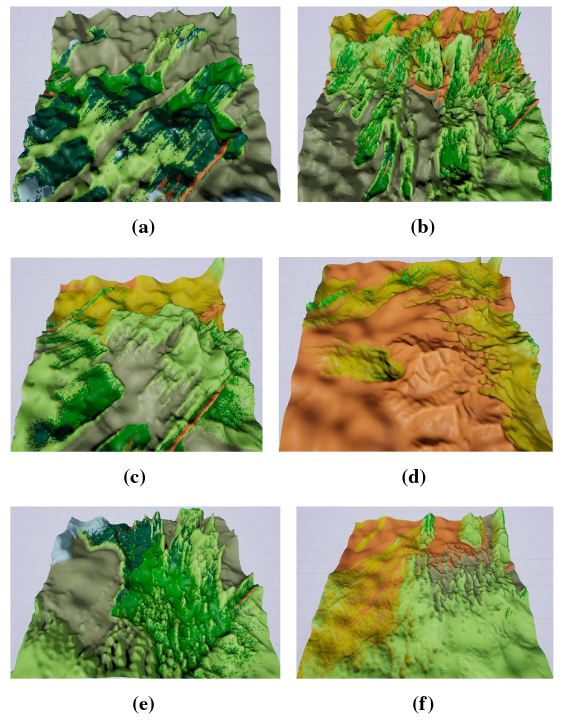
\includegraphics[width=0.4\linewidth]{images/Resultat_autobiomes.png}
        \caption{Un ensemble de terrains différents générés avec différents paramètres}
        \label{fig:enter-label}
    \end{figure}

    \paragraph{Conclusion} Ce papier présente une méthode intéressante pour la génération de terrain et de placement d'objets mais nous n'avons pas décidé de suivre cette méthode pour notre projet, celle ci est complexe et les résultats présentés ne nous ont pas convaincus. En effet pour une méthode qui met l'accent sur le réalisme nous trouvons les résultats trop aléatoires et peu esthétiques.
    Nous avons quand même utilisé certaines idées comme la table en fonction de l'élévation et de l'humidité pour les biomes.



    
        \subsubsection{papier 2 UI \cite{UIpaper}}

        \subsubsection{papier 3 DTM \cite{DTMpaper}}
        \subsubsection{papier 4}